\chapter{Introdução}

\section{Motivação e contexto}

\subsection{Materiais compósitos e sua relevância na engenharia}

Os materiais compósitos são definidos pela combinação de dois ou mais componentes macroscópicos diferentes, com o objetivo de obter propriedades físicas e mecânicas superiores às dos materiais homogêneos tradicionais \cite{RMJones2018}. O objetivo principal dessa classe de materiais reside no fato de que a resposta mecânica do sistema resultante não pode ser prevista a partir de nenhum de seus constituintes isolados, pois surge a partir da interação entre as fases que o compõem \cite{PartonReport}. Tal característica confere aos compósitos uma alta capacidade de ajuste de propriedades (rigidez, resistência específica, tenacidade, condutividade térmica, etc.), tornando-os indispensáveis em setores que impõem restrições simultâneas e conflitantes de desempenho estrutural e otimização de massa.

Na engenharia moderna, a utilização dessas estruturas é fundamental em setores que exigem alta resistência mecânica aliada à redução de peso, como as indústrias aeroespacial, automotiva, química e naval. Neste contexto, duas configurações estruturais concentram especial relevância tecnológica: os vasos de pressão de múltiplas camadas reforçados por fibra (\textit{Composite Overwrapped Pressure Vessels}, COPVs), amplamente empregados no armazenamento leve e seguro de gases sob altíssima pressão \cite[p.~1]{Zhang2022}, e os risers flexíveis utilizados em sistemas de produção de petróleo e gás em águas ultraprofundas sob solicitações combinadas de tração, flexão e pressão hidrostática externa \cite{Liu2026}. Ambas as aplicações operam sob condições severas de carregamento, com pressões internas elevadas e solicitações mecânicas cíclicas, exigindo modelos matemáticos e numéricos capazes de reproduzir com fidelidade a resposta mecânica local e global do componente.

Dentre as configurações cilíndricas multicamadas, a alternância periódica de fases metálicas distintas (cilindros bimetálicos) constitui um modelo representativo fundamental tanto para estruturas de engenharia que combinam resistência e leveza quanto para o desenvolvimento e validação de metodologias multiescala. No presente trabalho, investiga-se um cilindro composto pela alternância radial periódica de aço carbono estrutural (fase de elevada rigidez e contenção de pressão, com propriedades nominais equivalentes ao aço ASTM A516 Grau 70) e liga de alumínio estrutural (fase de baixa densidade, compatível com a liga AA 6061-T6). Esta combinação fundamenta-se em dois pilares:
\begin{enumerate}
    \item \textbf{Justificativa de engenharia e alívio de peso:} A substituição parcial do aço pelo alumínio ($\rho_{\text{alu}} \approx 2.700 \, \text{kg/m}^3$ contra $\rho_{\text{aço}} \approx 7.800 \, \text{kg/m}^3$) permite expressiva redução de massa estrutural (superior a $30\%$ para composições volumétricas simétricas), preservando a capacidade de sustentação de carga assegurada pelo módulo de elasticidade e limite de escoamento superiores do aço;
    \item \textbf{Justificativa físico-matemática e micromecânica:} O par bimetálico aço--alumínio estabelece uma razão de rigidez elástica severa ($E_{\text{aço}}/E_{\text{alu}} \approx 200/70 \approx 2{,}86$). Este contraste marcante cria um cenário ideal de \textit{benchmark} para desafiar teorias analíticas e métodos computacionais, evidenciando as descontinuidades de gradientes de deformação e os saltos de tensões nas interfaces que inviabilizam teorias clássicas simplificadas.
\end{enumerate}

O comportamento mecânico dessas estruturas heterogêneas é governado pela interação entre suas fases constituintes em múltiplas escalas. Uma análise fidedigna deve integrar informações que se estendem desde a microestrutura — onde se definem a geometria da célula unitária e as propriedades de cada lâmina individualmente — até o nível macroscópico, no qual o vaso de pressão como um todo é dimensionado e verificado \cite{PartonReport}. Essa necessidade de trânsito contínuo e consistente entre escalas espaciais distintas configura o chamado \textbf{problema multiescala}, cujo tratamento analítico e computacional constitui o núcleo temático deste trabalho.

\subsection{O desafio computacional do MEF e a abordagem assintótica}

O Método dos Elementos Finitos (MEF) constitui, atualmente, a ferramenta numérica predominante na análise de estruturas sólidas e compósitas. Contudo, sua aplicação direta a meios com propriedades rapidamente oscilantes — característicos de compósitos com dezenas ou centenas de microcamadas periódicas — impõe uma exigência computacional crítica: a malha de discretização espacial deve ser suficientemente refinada para posicionar nós e arestas ao longo de cada uma das interfaces e capturar os severos gradientes locais em escala microscópica $l$ \cite{Guinovart2024}. À medida que o número de camadas aumenta, a dimensão dos sistemas algébricos lineares resultantes torna-se proibitiva em termos de consumo de memória RAM e tempo de processamento.

Como alternativa analítica rigorosa a este gargalo computacional, o Método de Homogeneização Assintótica (MHA) propõe substituir o meio heterogêneo original por um material contínuo equivalente macroscopicamente homogêneo, cujas propriedades constitutivas efetivas encapsulam com exatidão os efeitos médios da microestrutura periódica \cite{bakhvalov1989}. Desta forma, o MHA permite resolver o problema estrutural global em uma malha contínua e suave, desacoplando a escala global do número real de lâminas do componente.

\subsection{Problema multiescala e o princípio de separação de escalas}

A modelagem analítica de componentes micro-heterogêneos fundamenta-se no \textbf{princípio da separação de escalas} e na \textbf{hipótese do contínuo}. O princípio de separação de escalas postula que haja uma distinção nítida entre as dimensões microscópica e macroscópica, expressa pelo parâmetro geométrico adimensional $\epsilon$, definido por \cite[p.~17]{bakhvalov1989} como a razão entre os comprimentos característicos da microescala $l$ (associado ao período da célula unitária) e da macroescala $L$ (associado à espessura da parede do vaso de pressão):
\begin{equation}
  \epsilon = \frac{l}{L}
  \label{eq:epsilon_definicao}
\end{equation}

A \autoref{fig:separacao_escalas} ilustra esquematicamente o conceito de transição entre as escalas macroscópica, microscópica e a representação periódica contínua:

\begin{figure}[htbp]
    \centering
    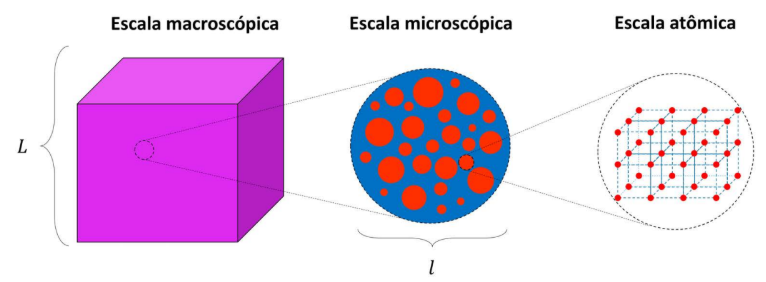
\includegraphics[width=0.75\linewidth]{capitulos/imagens/Separação de escalas.png}
    \caption{Representação esquemática do princípio da separação de escalas e do parâmetro geométrico adimensional $\epsilon$.}
    \label{fig:separacao_escalas}
\end{figure}

A validade física e matemática das abordagens multiescala repousa sobre a condição $0 < \epsilon \ll 1$. Quando o parâmetro $\epsilon$ é suficientemente pequeno, torna-se possível desacoplar os problemas nas duas escalas espaciais: a coordenada macroscópica lenta $\mathbf{x}$ e a coordenada microscópica rápida $\mathbf{y} = \mathbf{x}/\epsilon$, responsável por descrever as oscilações periódicas locais da solução dentro da célula unitária \cite{bakhvalov1989}. 

Para a condução da modelagem analítica, postula-se uma \textit{Solução Assintótica Formal} (SAF) expressa como uma série de potências do parâmetro $\epsilon$: (conforme desenvolvido no Capítulo 3, Seção 3.2).
\begin{equation}
  \mathbf{u}^{(\infty)}(\mathbf{x}, \epsilon) = \mathbf{u}^0(\mathbf{x}) + \epsilon \mathbf{u}^1(\mathbf{x}, \mathbf{y}) + \epsilon^2 \mathbf{u}^2(\mathbf{x}, \mathbf{y}) + \dots
  \label{eq:saf_expansao}
\end{equation}

A substituição desta expansão nas equações governantes de equilíbrio mecânico e a segregação dos termos por ordens de magnitude em $\epsilon$ decompõem o problema original em uma hierarquia bem definida:
\begin{enumerate}
    \item Um \textit{problema local sobre a célula unitária}, que fornece as funções de perturbação elástica e permite calcular de forma analítica fechada os \textbf{coeficientes elásticos efetivos} do cilindro homogeneizado;
    \item Um \textit{problema macroscópico equivalente}, formulado sobre o domínio contínuo global e governado pelas propriedades homogeneizadas.
\end{enumerate}

No formalismo do MHA, a aproximação de ordem zero ($\mathbf{u}^0$) descreve com precisão a resposta macroscópica média de deslocamentos da estrutura. O termo corretor de primeira ordem $\epsilon \mathbf{u}^1(\mathbf{x}, \mathbf{y})$, por sua vez, é responsável por capturar as flutuações e os gradientes locais decorrentes da heterogeneidade. No presente trabalho, a formulação analítica do MHA é desenvolvida até a determinação fechada das propriedades constitutivas efetivas e a resolução do campo macroscópico $\mathbf{u}^0$, enquanto a implementação computacional da reconstrução analítica ponto a ponto das flutuações locais via $\epsilon \mathbf{u}^1$ é delineada formalmente como etapa de extensão em trabalhos futuros, sendo a validação dos campos locais conduzida comparativamente frente ao modelo detalhado em elementos finitos.

\section{Objetivo geral}

O objetivo geral deste trabalho é realizar uma análise mecânica multiescala de vasos de pressão cilíndricos multicamadas com periodicidade radial, estabelecendo uma comparação sistemática e quantitativa de precisão e eficiência computacional entre o Método dos Elementos Finitos (MEF), empregado como modelo detalhado de referência, e o Método de Homogeneização Assintótica (MHA), empregado como formulação analítica equivalente, tendo a clássica solução analítica exata de Lamé como padrão fundamental de calibração e verificação do solucionador numérico para o caso homogêneo.

\section{Objetivos específicos}

Para atingir o objetivo geral, definem-se os seguintes objetivos específicos:

\begin{enumerate}
  \item \textbf{Formular o problema de equilíbrio mecânico do cilindro compósito microperiódico} em coordenadas cilíndricas tridimensionais sob hipótese de simetria de revolução (axissimetria) e deformação plana generalizada, deduzindo a equação diferencial ordinária governante unidimensional radial;
  \item \textbf{Aplicar o formalismo do MHA ao problema formulado}, deduzindo as equações diferenciais recorrentes, as condições de contorno de célula unitária, as funções corretoras locais e a equação governante homogeneizada macroscópica;
  \item \textbf{Deduzir analiticamente os coeficientes elásticos efetivos} para a configuração cilíndrica bilaminada bimetálica (aço--alumínio), correlacionando os resultados obtidos com os limites clássicos de Reuss (média harmônica radial) e a formulação de meios estratificados de Backus (rigidez circunferencial e módulo de cisalhamento efetivo);
  \item \textbf{Implementar e calibrar um solucionador numérico axissimétrico} baseado na plataforma de elementos finitos em código aberto FEniCS, validando a formulação variacional fraca através da clássica solução analítica de Lamé para cilindros homogêneos de parede grossa;
  \item \textbf{Comparar quantitativamente a precisão e a eficiência computacional} entre a solução macroscópica homogeneizada pelo MHA e a solução numérica detalhada do MEF, avaliando o comportamento assintótico das descontinuidades de gradiente nas interfaces, a redução dos erros numéricos e o ganho de tempo de processamento (\textit{speedup}) em função do aumento do número de camadas do vaso.
\end{enumerate}

\section{Organização e limitações do trabalho}

O presente trabalho está estruturado em seis capítulos:
\begin{itemize}
    \item O \textbf{Capítulo 1 (Introdução)} contextualiza a pesquisa, justifica a seleção dos materiais e estabelece os objetivos e delimitações do estudo;
    \item O \textbf{Capítulo 2 (Revisão Bibliográfica)} aborda os critérios normativos para vasos de pressão (ASME Seção VIII e NR-13), a mecânica dos materiais compósitos anisotrópicos, as teorias cinemáticas de placas/cascas, os mecanismos de descontinuidade em interfaces e os fundamentos do MHA e do MEF;
    \item O \textbf{Capítulo 3 (Formulação Matemática e Homogeneização)} apresenta o equacionamento analítico do equilíbrio axissimétrico em coordenadas cilíndricas e desenvolve a dedução detalhada do MHA e dos coeficientes constitutivos efetivos;
    \item O \textbf{Capítulo 4 (Metodologia e Simulação Numérica)} descreve a implementação computacional do modelo de elementos finitos axissimétrico no ambiente FEniCS, detalhando a discretização da malha estruturada, as funções de interpolação e o mapeamento periódico das propriedades mecânicas;
    \item O \textbf{Capítulo 5 (Resultados e Discussões)} expõe a validação analítica via solução de Lamé, a análise comparativa de deslocamentos e tensões entre MEF e MHA, o comportamento assintótico de convergência e a avaliação de eficiência computacional e alívio de peso estrutural;
    \item O \textbf{Capítulo 6 (Conclusões e Trabalhos Futuros)} sintetiza as principais contribuições técnicas do estudo e delineia propostas para extensões da pesquisa.
\end{itemize}

\subsection{Delimitação do escopo e limitações do modelo}

A fim de assegurar o rigor e a consistência da modelagem matemática e numérica desenvolvida, o escopo deste trabalho está delimitado sob as seguintes premissas e simplificações físicas:
\begin{itemize}
    \item \textbf{Regime mecânico e cinemático:} Considera-se comportamento elástico linear, puramente isotrópico em nível de subcamada homogênea individual, operando sob a hipótese de deformações e deslocamentos infinitesimais;
    \item \textbf{Condição cinemática de extremidade:} Adota-se o estado de deformação plana generalizada ($\epsilon_{zz} = \text{constante}$), condizente com cilindros de comprimento axial longo submetidos a carregamento uniforme de pressão interna de regime permanente ($P_{\text{int}} = 30 \, \text{MPa}$);
    \item \textbf{Condições interfaciais ideais:} Assume-se aderência e contato mecânico perfeito entre as lâminas adjacentes de aço e alumínio, com continuidade estrita de deslocamentos radiais e tensões de tração normais, desconsiderando fenômenos de delaminação, escorregamento interfacial, plasticidade ou propagação de trincas;
    \item \textbf{Condições térmicas e ambientais:} A análise é estritamente isotérmica, desconsiderando efeitos de gradientes de temperatura, dilatação térmica diferencial residual de fabricação ou mecanismos de corrosão galvânica entre as fases metálicas;
    \item \textbf{Alcance da implementação do MHA:} O modelo de homogeneização analítico é aplicado à dedução das constantes constitutivas efetivas e à resolução da resposta macroscópica de deslocamento médio ($\mathbf{u}^0$), sendo a implementação numérica computacional da reconstrução pós-processada ponto a ponto do campo local corretivo ($\epsilon \mathbf{u}^1$) reservada para investigações e trabalhos futuros.
\end{itemize}
